\chapter{Aeroelastic study} \label{chap:aeroelastic}

  %Intro
  In the present chapter, the compliant design for the wing-box is embedded into a full wing model. A pressure field is then introduced to simulate the pressure distribution obtained from fluid-airfoil interaction. Using this model, a weakly coupled aeroelastic study is performed. 

  \section{Wing model} \label{sec:wingModel_aeroelastic}

    The wing model is described in the present section. This wing features a NACA 0012 airfoil and a wing-box comprised by two spars, it also has its chord constant throughout the whole span. The wing geometrical characterization is completed by the span $s$, the chord length $c_0$, and the position of the front and rear spars of the wing-box, $c_1$ and $c_2$, respectively and in the chordwise direction. These two last parameters are expressed in dimensionless form as a function of $c_0$, resulting on $\hat{c}_1 = c_1 /c_0$ for the front spar and in $\hat{c}_2 = c_2 /c_0$ for the rear spar. The computational model built only comprises half of the span. This geometrical description of the wing is also graphically shown in Figure \ref{fig:wing-dim}. 

    \begin{figure}[!htpb]
      \centering
      \subfigure[Airfoil dimensions.]{\label{fig:wing-dim1}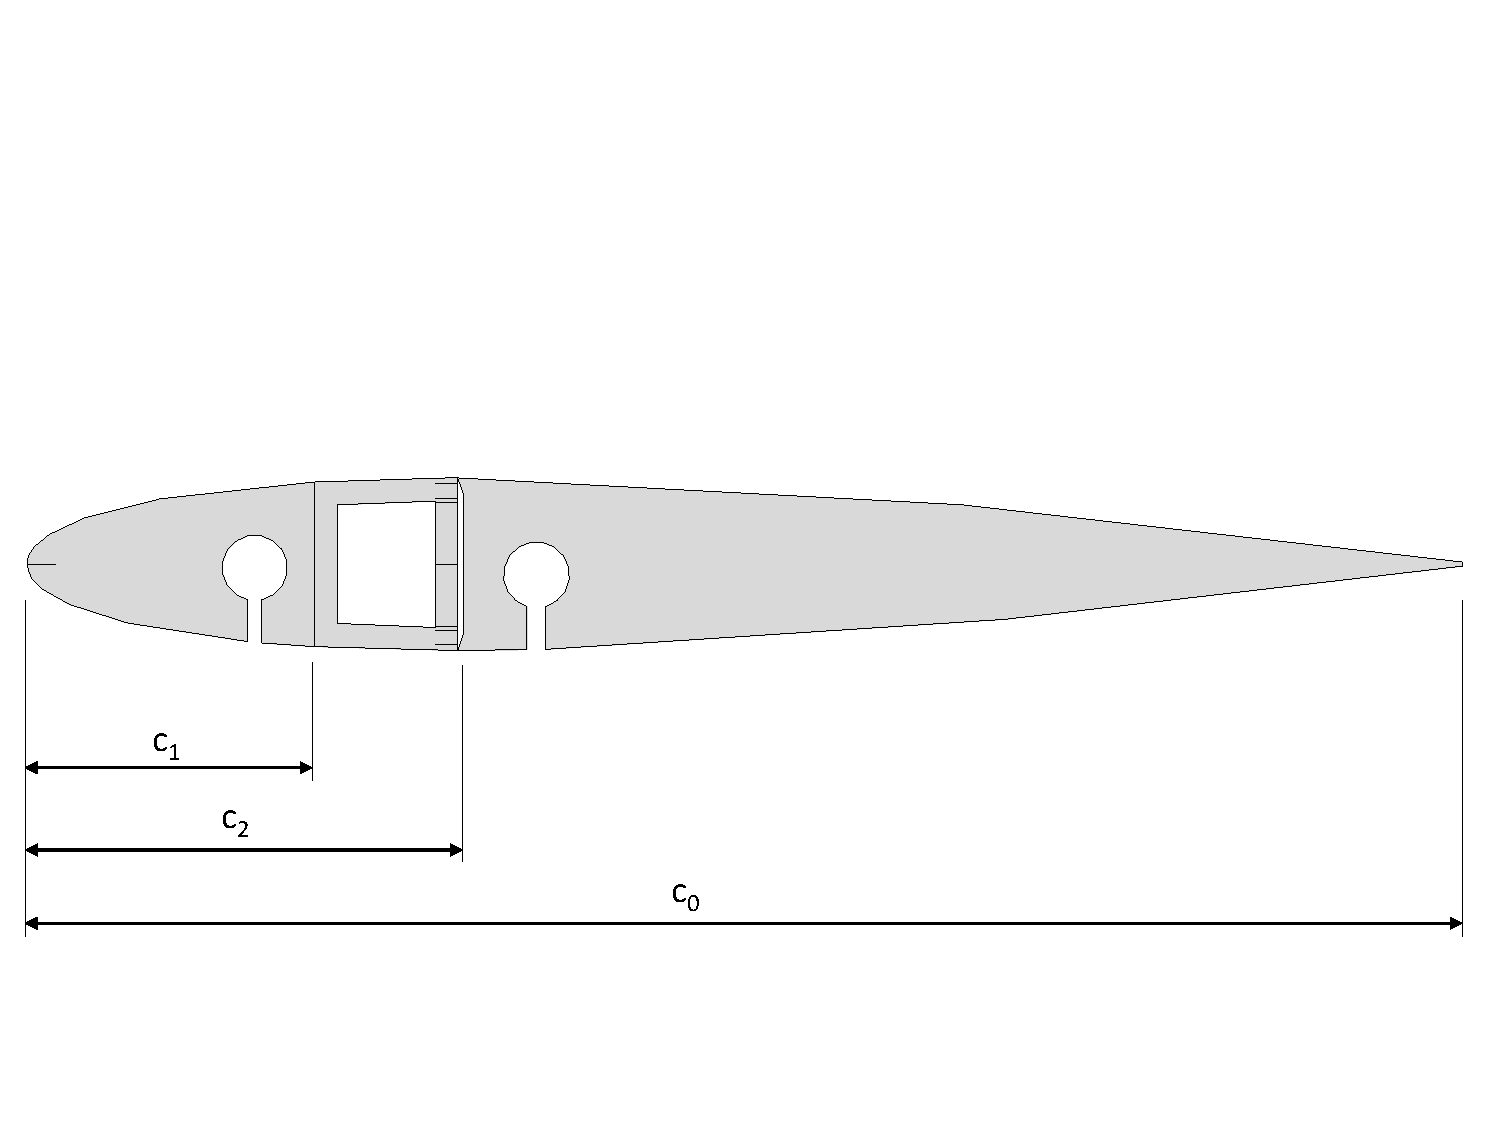
\includegraphics[width=0.6\textwidth]{figures/wing-model/airfoilDim1}} \qquad
      \subfigure[Wing span.]{\label{fig:wing-dim2}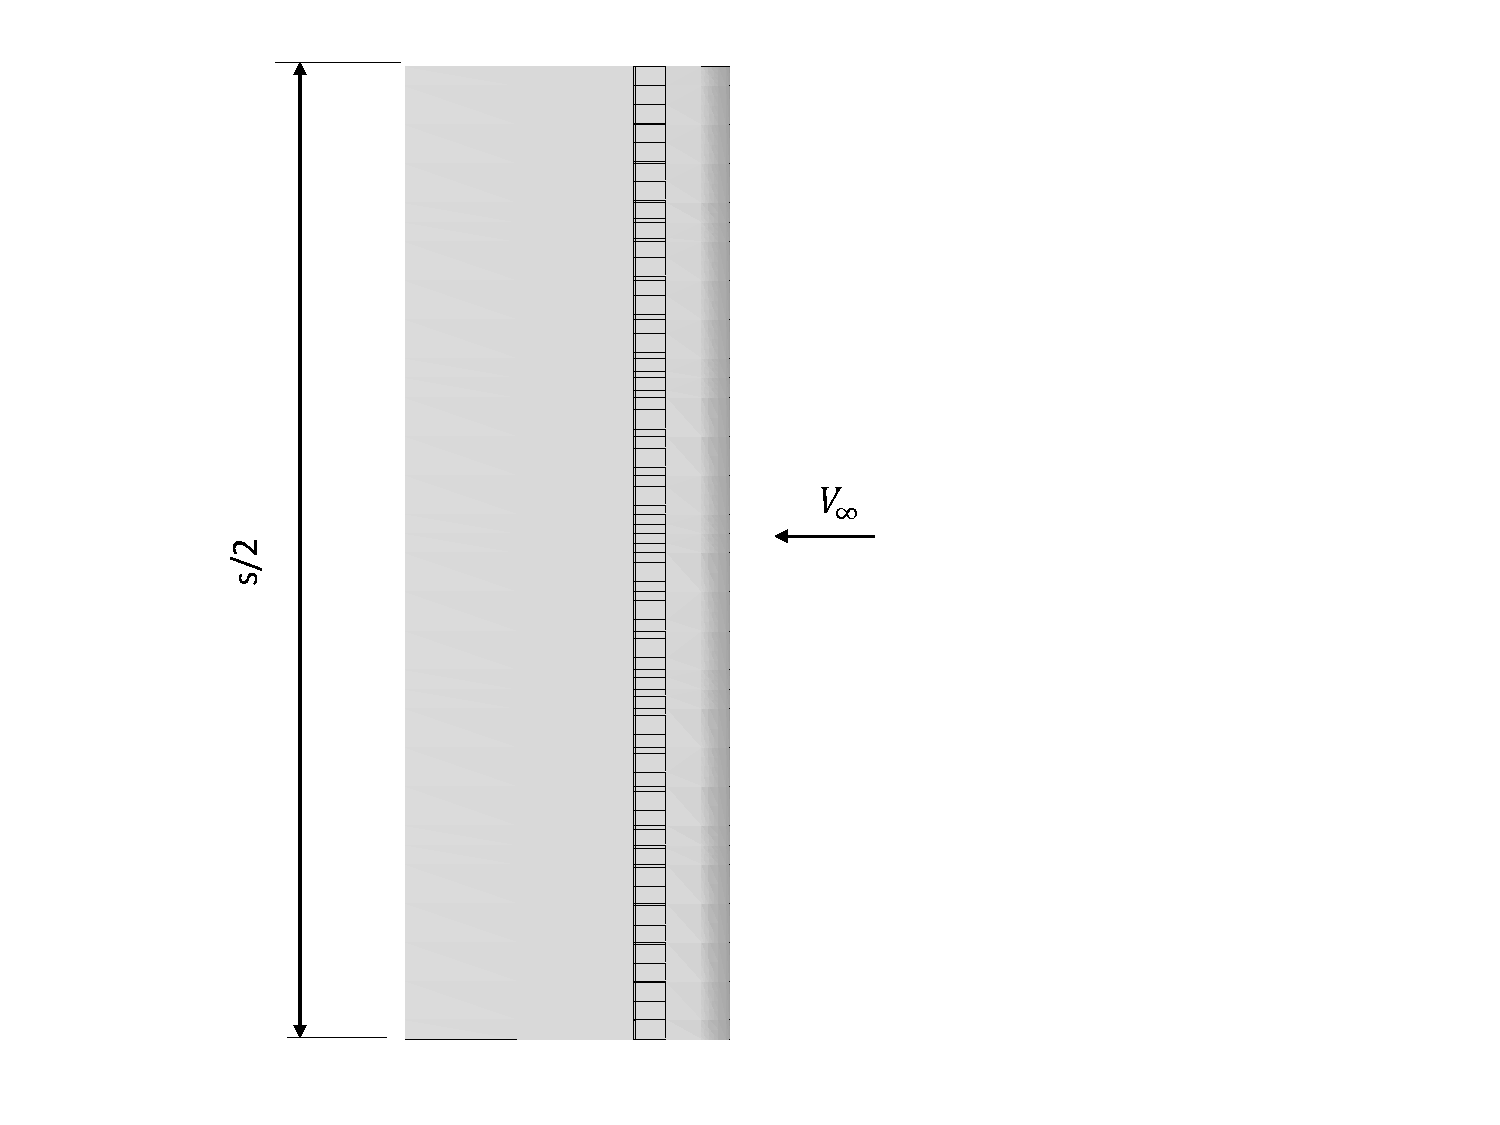
\includegraphics[width=0.3\textwidth]{figures/wing-model/airfoilDim2}}
      \caption[Wing geometrical characterization]{Wing and airfoil geometrical characterization. The airfoil is standard NACA 0012. The parameters are the span $s$, the chord length $c_0$, and the position of the front and rear spars of the wing-box, $c_1$ and $c_2$, respectively.}
      \label{fig:wing-dim}
    \end{figure}

    An overview of the computational model is shown in Figure \ref{fig:wing}. The boundary condition for wing is established through the wing-box which has all its degrees of freedom restrained at the root.

    \begin{figure}[!htpb]
      \centering
      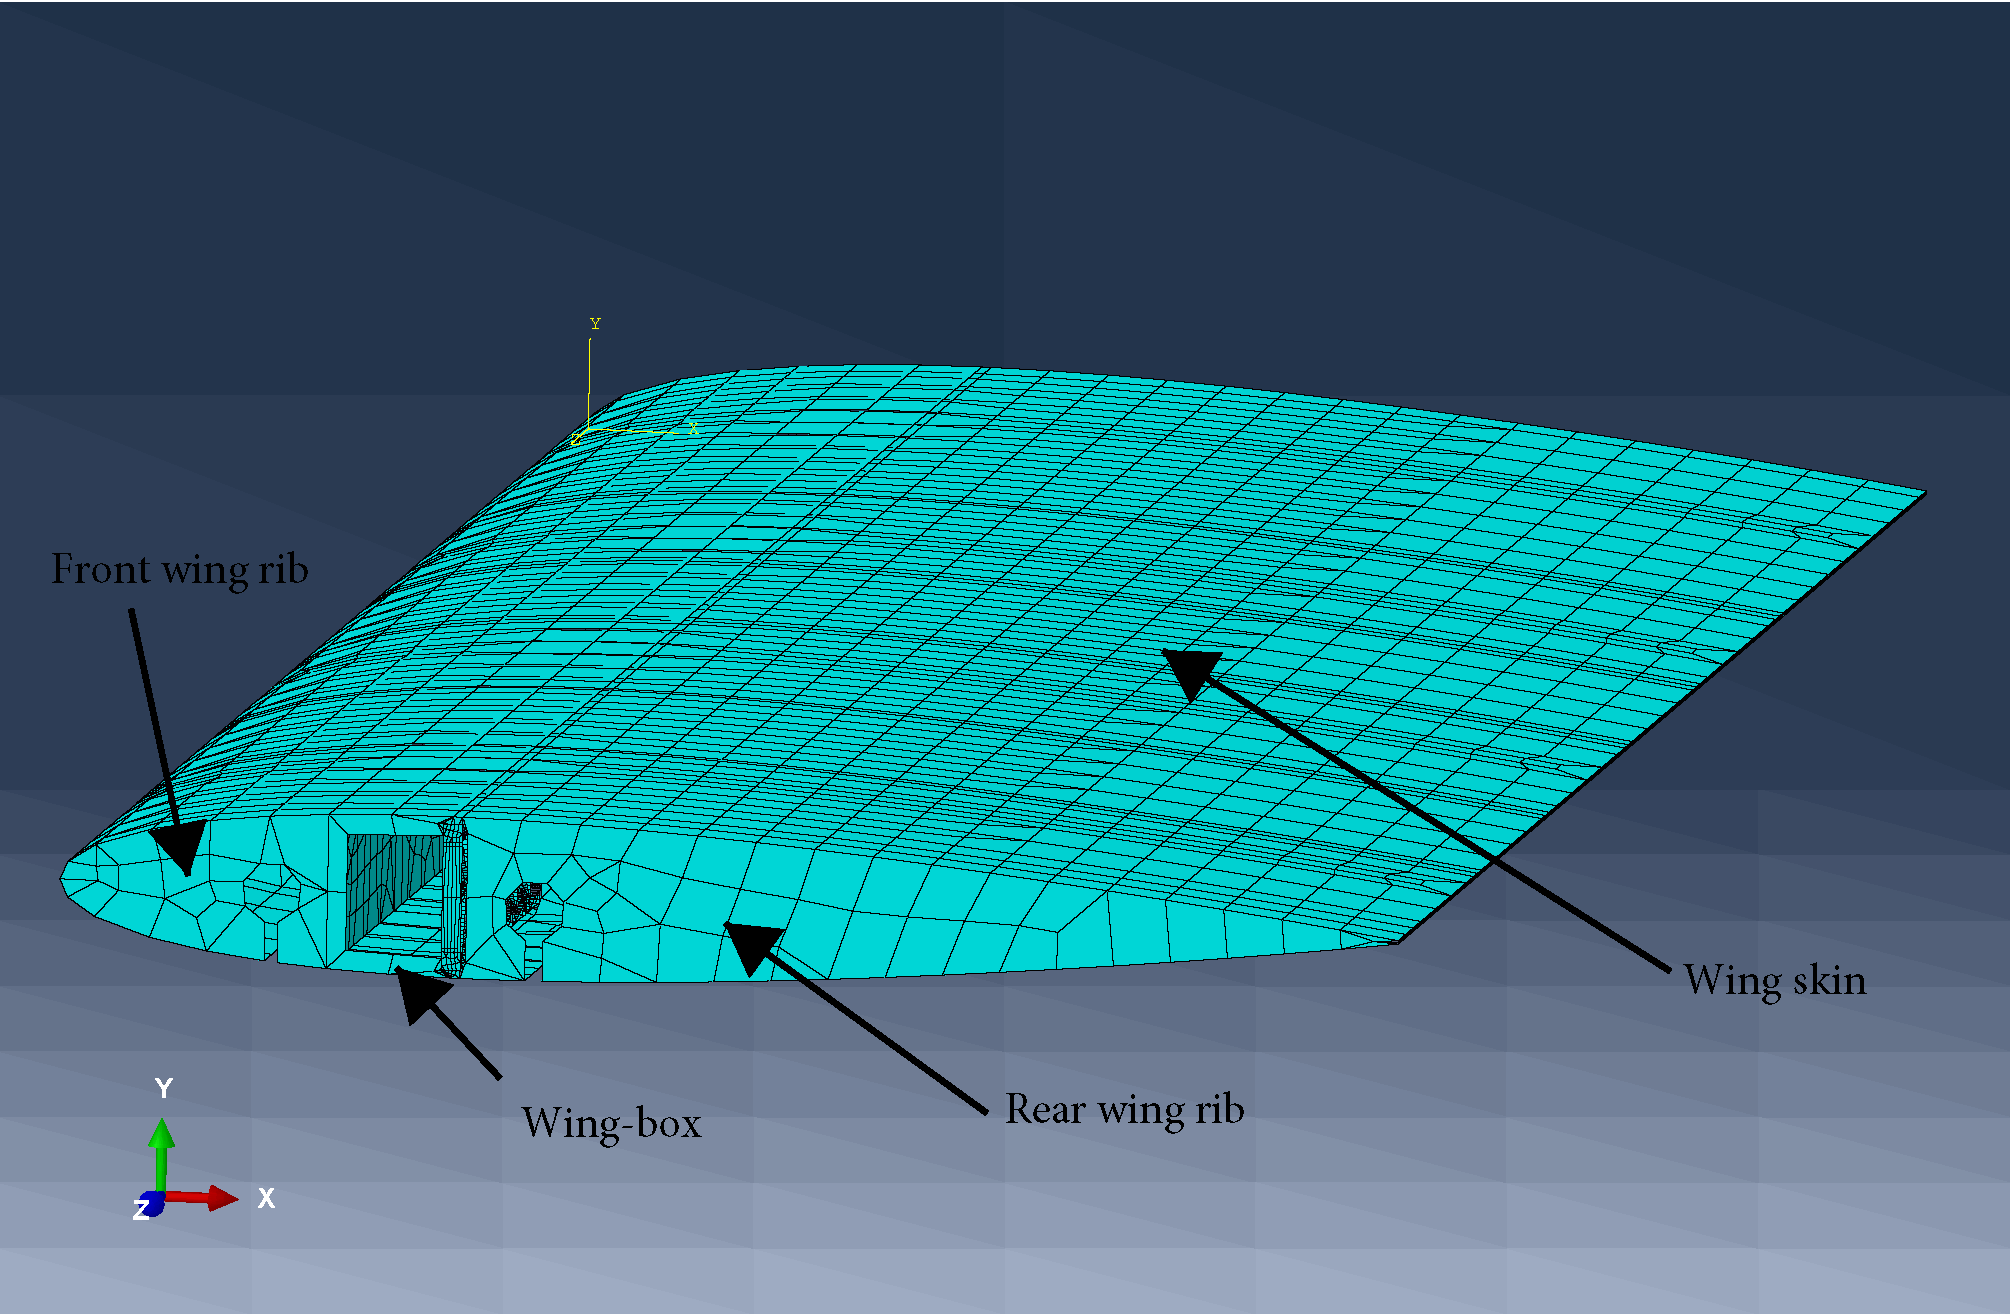
\includegraphics[width=0.7 \textwidth]{figures/wing-model/wing_correct}
      \caption[Overview of the wing FEM model embedded with the compliant wing-box design]{Overview of the wing FEM model embedded with the compliant wing-box design.}
      \label{fig:wing}
    \end{figure}

  \clearpage
  \section{Weakly coupled static aeroelastic analysis} \label{sec:aeroelastic_aeroelastic}
    % Parameters utilized
    % Desciption of the method

    In this section, the method followed to perform the weakly coupled aeroelastic analysis is described. 

    The pressure distribution field originated from the fluid-airfoil interaction is responsible of the forces applied into the wing model. This is the only source of forces introduced into the model. The pressure distribution is obtained using XFOIL$^{\textregistered}$ software and a lift line method developed at CMAS lab.

    The flight condition is determined by introducing the air velocity $V$, the air density $\rho$, the air dynamic viscosity $\mu$ and the angle of attack of the wing $\alpha_0$.

    Firstly, the given flight condition makes it possible to obtain the corresponding pressure distribution that it is applied to the wing skin. However, since the aeroelastic coupling between aerodynamic forces and the wing twist adaptation is expected to be nonlinear, it becomes necessary to introduce split the prescribed pressure load into small increments.

    At each of the increments mentioned previously, the magnitude of the pressure applied $p_{\mathrm{step}}$ into the wing skin is scaled to a fraction of the magnitude of the total prescribed pressure $P_{\mathrm{total}}$, at each coordinate $x$ and $y$, as shown in Equation \ref{eq:pressure}:
    %
    \begin{equation}
      P_{\mathrm{total}} = \sum_{i_{\mathrm{step}} = 1}^{n_{\mathrm{steps}}} p_{\mathrm{step}},
      \label{eq:pressure}
    \end{equation}
    %
    where $n_{\mathrm{steps}}$ is the total number of steps. The pressure applied at each each step is added to the one from previous steps conforming a stepped load introduction.

    At each of the increments, the wing deformation that is originated by the pressure distribution in the wing skin is obtained after convergence is achieved. After, the pressure distribution that corresponds to the next increment is introduced and a new deformation state is seek.

    The complete set of values of the parameters used in the model and in the aeroelastic analysis is shown in Table \ref{tab:parameters_aeroelastic}.

    \begin{table}[!htpb]
      \centering
      \begin{tabular}{|l|lll|}
      \hline
      \textbf{Parameter} & \multicolumn{1}{l|}{\textbf{Symbol}} & \multicolumn{1}{l|}{\textbf{Units}} & \textbf{Nominal value} \\ \hline \hline
      {\textbf{Wing and airfoil dimensions}} &  &  &  \\ \hline
      Span & \multicolumn{1}{l|}{$s$} & \multicolumn{1}{l|}{m} & 3 \\ \hline
      Chord length & \multicolumn{1}{l|}{$c_0$} & \multicolumn{1}{l|}{m} & 0.5 \\ \hline
      Dimensionless position of the front wing-box spar & \multicolumn{1}{l|}{$\hat{c}_1$} & \multicolumn{1}{l|}{} & 0.2 \\ \hline
      Dimensionless position of the rear wing-box spar & \multicolumn{1}{l|}{$\hat{c}_2$} & \multicolumn{1}{l|}{} & 0.3 \\ \hline
      Wall thickness for the wing ribs & \multicolumn{1}{l|}{$t_{\mathrm{wing,rib}}$} & \multicolumn{1}{l|}{mm} & 4 \\ \hline \hline
      {\textbf{Compliant spar design with lattice of chiral structures}} &  &  &  \\ \hline
      Number of unit cells in spanwise direction & \multicolumn{1}{l|}{$N$} & \multicolumn{1}{l|}{} & 52 \\ \hline
      Number of unit cells in transversal direction & \multicolumn{1}{l|}{$M$} & \multicolumn{1}{l|}{} & 2 \\ \hline
      Dimensionless ligament eccentricity (e/B) & \multicolumn{1}{l|}{$\epsilon_{\mathrm{chi}}$} & \multicolumn{1}{l|}{} & 0.01 \\ \hline
      Node radius & \multicolumn{1}{l|}{$r_{\mathrm{chi}}$} & \multicolumn{1}{l|}{mm} & 2.5355 \\ \hline
      Node depth & \multicolumn{1}{l|}{$B_{\mathrm{chi}}$} & \multicolumn{1}{l|}{mm} & 8 \\ \hline
      Ligament half length & \multicolumn{1}{l|}{$L_{\mathrm{chi}}$} & \multicolumn{1}{l|}{mm} & 14.486 \\ \hline
      Thickness & \multicolumn{1}{l|}{$t_{\mathrm{chi}}$} & \multicolumn{1}{l|}{mm} & 0.4 \\ \hline \hline
      {\textbf{Flight condition}} &  &  &  \\ \hline
      Free-stream air speed & \multicolumn{1}{l|}{$V$} & \multicolumn{1}{l|}{m/s} & 30 \\ \hline
      Angle of attack of the wing & \multicolumn{1}{l|}{$\alpha_0$} & \multicolumn{1}{l|}{deg} & 8 \\ \hline
      Air density & \multicolumn{1}{l|}{$\rho$} & \multicolumn{1}{l|}{kg/m$^3$} & 1.225 \\ \hline
      Air dynamic viscosity & \multicolumn{1}{l|}{$\mu$} & \multicolumn{1}{l|}{N s/m$^2$} & \notcien{1.789}{-5} \\ \hline \hline
      {\textbf{Material for the chiral lattice (ABS)}} &  &  &  \\ \hline
      Young's modulus & \multicolumn{1}{l|}{$E_{\mathrm{chi}}$} & \multicolumn{1}{l|}{N/mm$^2$} & 3100 \\ \hline
      Poisson's ratio & \multicolumn{1}{l|}{$\nu_{\mathrm{chi}}$} & \multicolumn{1}{l|}{} & 0.3 \\ \hline \hline
      {\textbf{Material for the wing skin (CFRP)}} &  &  &  \\ \hline
      Ply lay-up description & \multicolumn{1}{l|}{} & \multicolumn{1}{l|}{} & $[0_2,90_2]_{\mathrm{s}}$ \\ \hline
      Ply thickness & \multicolumn{1}{l|}{$t_{\mathrm{ply}}$} & \multicolumn{1}{l|}{mm} & 0.125 \\ \hline
      Young's modulus 0$^{\circ}$ & \multicolumn{1}{l|}{$E_{\mathrm{ply,1}}$} & \multicolumn{1}{l|}{N/mm$^2$} & 135000 \\ \hline
      Young's modulus 90$^{\circ}$ & \multicolumn{1}{l|}{$E_{\mathrm{ply,2}}$} & \multicolumn{1}{l|}{N/mm$^2$} & 10000 \\ \hline
      Major Poisson's ratio & \multicolumn{1}{l|}{$\nu_{\mathrm{ply}}$} & \multicolumn{1}{l|}{} & 0.3 \\ \hline
      In-plane shear modulus & \multicolumn{1}{l|}{$G_{\mathrm{ply,12}}$} & \multicolumn{1}{l|}{N/mm$^2$} & 5000 \\ \hline
      Transverse shear modulus & \multicolumn{1}{l|}{$G_{\mathrm{ply,13}}$} & \multicolumn{1}{l|}{N/mm$^2$} & 5000 \\ \hline
      Transverse shear modulus & \multicolumn{1}{l|}{$G_{\mathrm{ply,23}}$} & \multicolumn{1}{l|}{N/mm$^2$} & 3846 \\ \hline
      {\textbf{Material for the wing rib (Aluminum)}} &  &  &  \\ \hline
      Young's modulus & \multicolumn{1}{l|}{$E_{\mathrm{wing,rib}}$} & \multicolumn{1}{l|}{N/mm$^2$} & 69000 \\ \hline
      Poisson's ratio & \multicolumn{1}{l|}{$\nu_{\mathrm{wing,rib}}$} & \multicolumn{1}{l|}{} & 0.3269 \\ \hline
      \end{tabular}
      \caption[Parameters that define the wing model and the aeroelastic analysis]{Parameters that define the wing model and the aeroelastic analysis. The table includes the wing and airfoil geometrical dimensions, the internal parameters for the lattice of chiral structures and the flight condition. Furthermore, the description of the materials used in the different parts of the model is also included.}
      \label{tab:parameters_aeroelastic}
    \end{table}

    \clearpage
    \subsection{Results from simulations} \label{subsec:results_aeroelastic}

      The results from the simulations carried out with the model described in Table \ref{tab:parameters_aeroelastic} are presented below. The total pressure load given by the considered flight condition is applied in ten individual steps. The evolution of the wing twist deformation at each of these steps in shown in Figure \ref{fig:twist_perIter_s3_V30}. It can be seen that the wing twist deformation increases as the velocity increases. Moreover, it can be sen that the number of iterations required to achieve the convergence at each of the steps increases as the air velocity increases.

      When showing the achieved wing twist as a function of the current airspeed that is equivalent to the applied pressure, the Figure \ref{fig:twist_perV_s3_V30} is produced. Here, the response after executing nonlinear and linear simulations are both displayed and compared. It can be seen that the agreement between the two responses decreases as the velocity increases.

      Furthermore, the deformed wing model displaying the wing tip twist can be seen in Figure \ref{fig:bucklingWing3}. In Figure \ref{fig:bucklingWing2}, a detailed cut view in the spanwise direction of the wing shows the buckling field in the spar of chiral structures.

      \begin{figure}[!htpb]
        \centering
        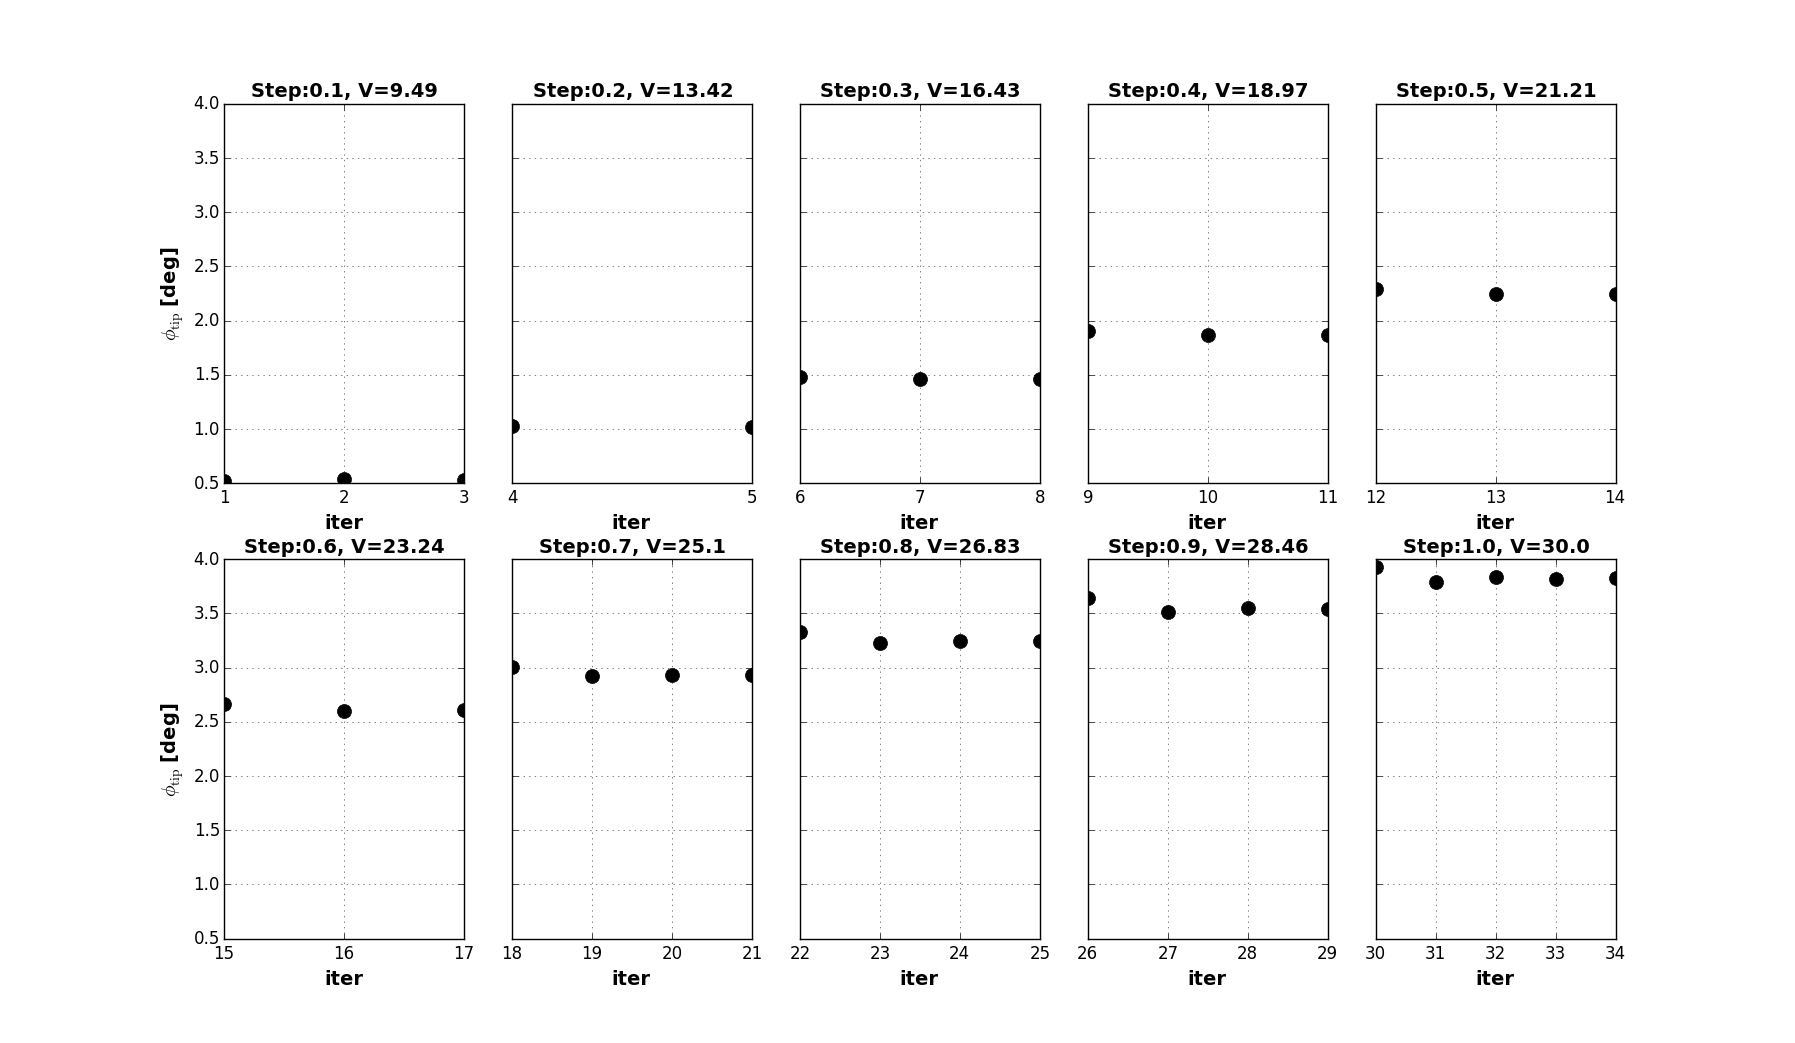
\includegraphics[width=0.95 \textwidth]{figures/wing-model/twist_perIter_s3_V30}
        \caption[Wing twist adaptation at each step]{Wing twist adaptation at each step. Results show the wing twist deformation increases as the velocity increases. Also, it can be sen that the number of iterations required to achieve the convergence at each of the steps increases as the air velocity increases.}
        \label{fig:twist_perIter_s3_V30}
      \end{figure}

      \begin{figure}[!htpb]
        \centering
        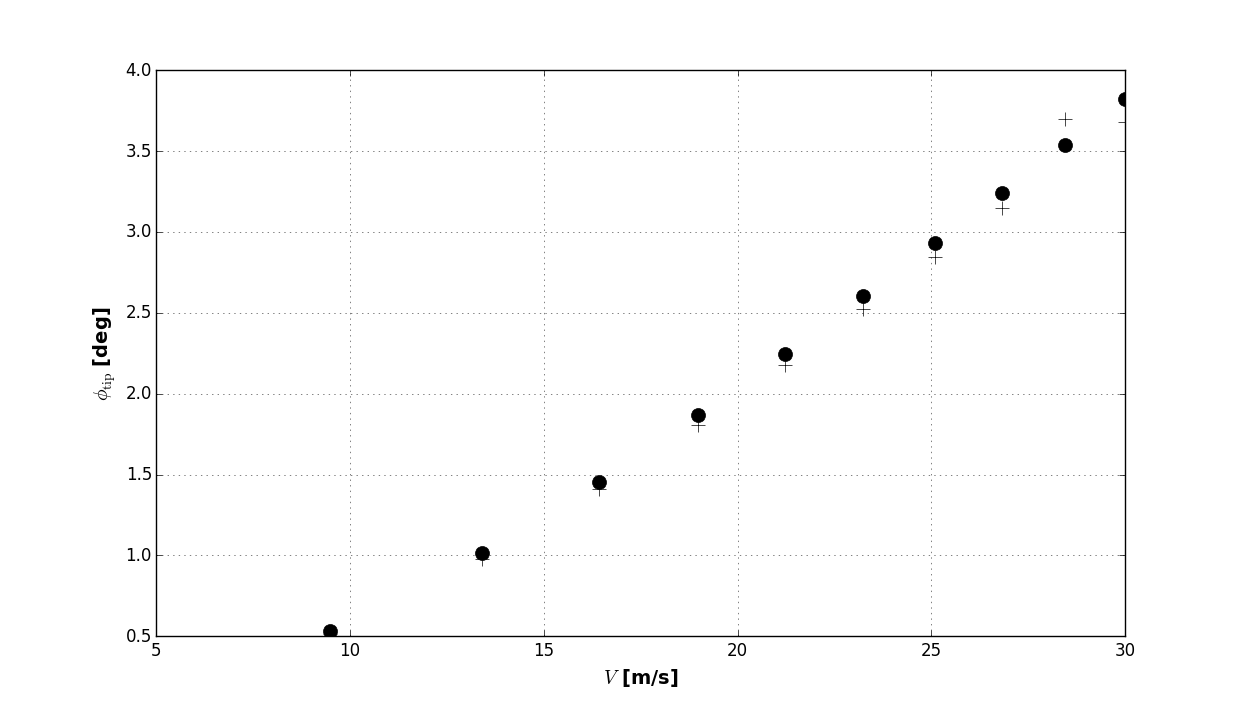
\includegraphics[width=0.8 \textwidth]{figures/wing-model/twist_perV_s3_V30}
        \caption[Wing twist as a function of the air velocity]{Wing twist as a function of the air velocity that corresponds to each pressure load applied at each step. The filled dots represent the response in twist for the nonlinear simulation while the crosses represent the response for the linear simulation. It can be seen that the agreement between the two responses decreases as the velocity increases.}
        \label{fig:twist_perV_s3_V30}
      \end{figure}

      \begin{figure}[!htpb]
        \centering
        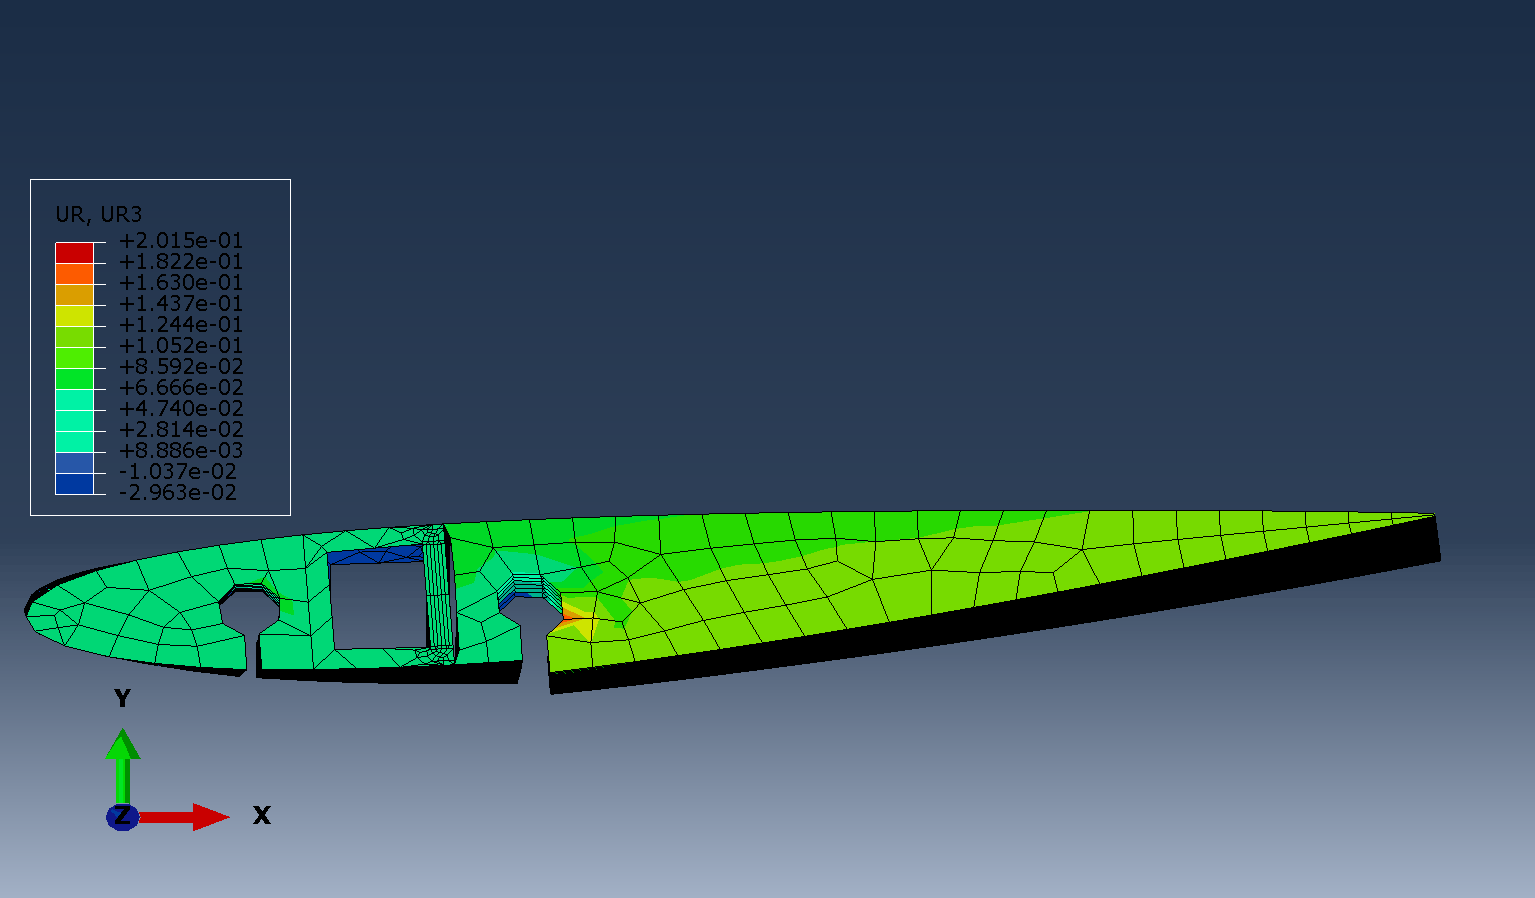
\includegraphics[width=0.8 \textwidth]{figures/wing-model/bucklingWing3}
        \caption[Deformed wing model displaying the wing twist deformation]{Deformed wing model displaying the wing twist deformation. At the stage shown in the figure, all the prescribed load for the considered flight condition has been applied.}
        \label{fig:bucklingWing3}
      \end{figure}

      \begin{figure}[!htpb]
        \centering
        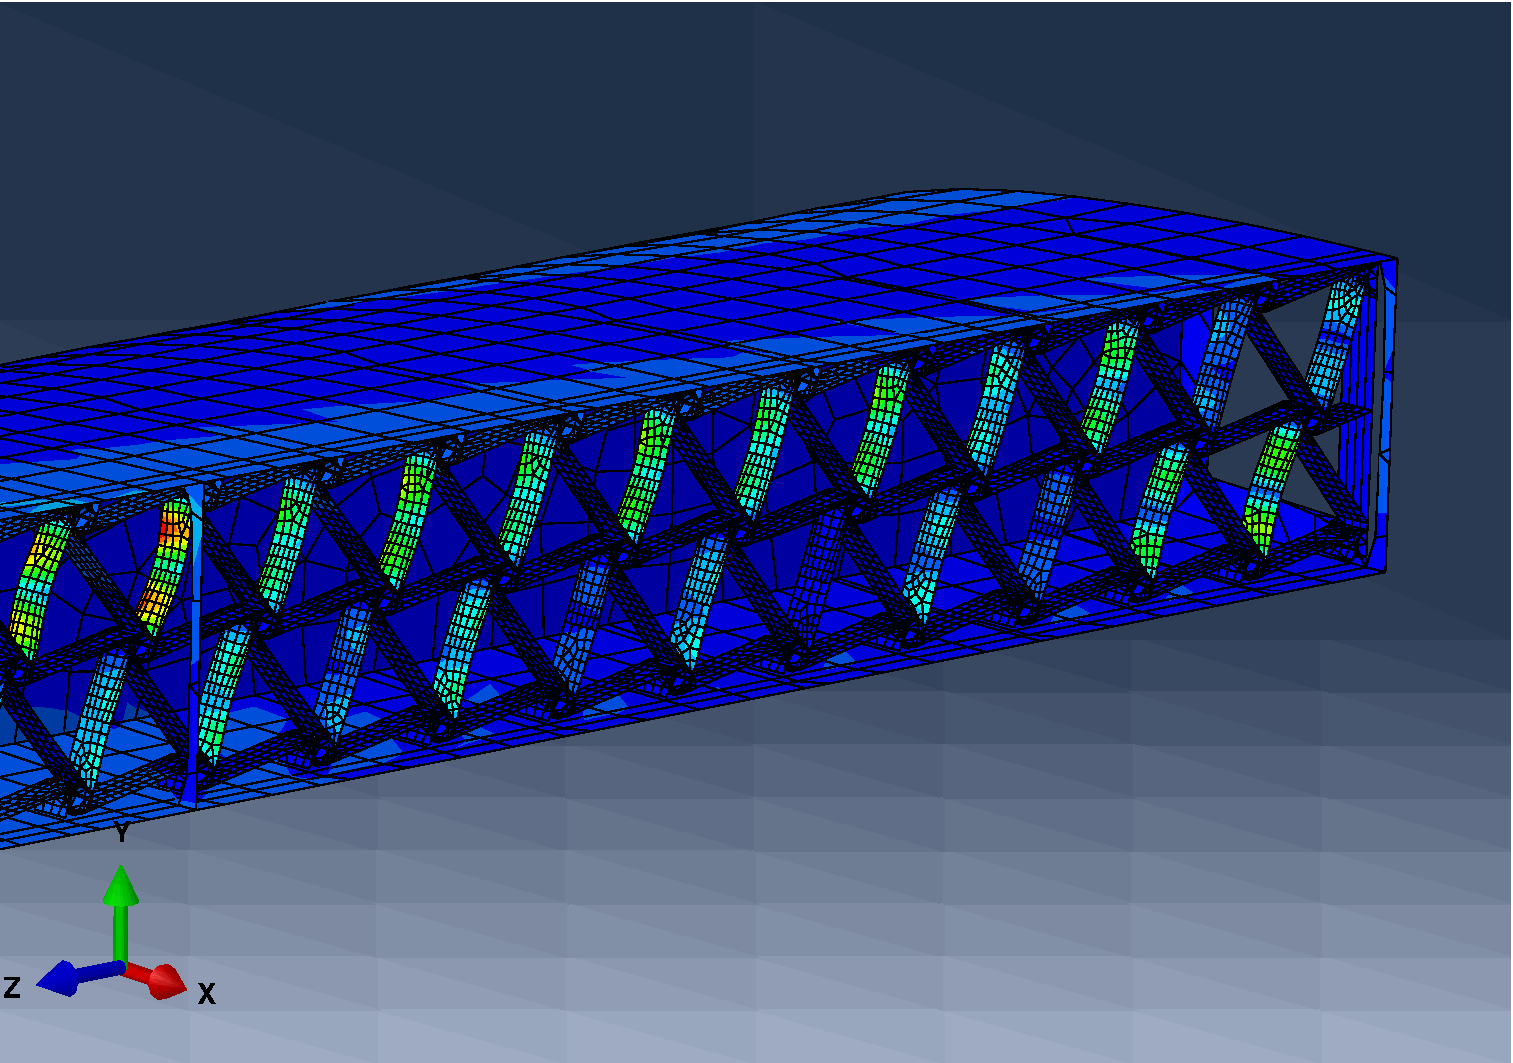
\includegraphics[width=0.8 \textwidth]{figures/wing-model/bucklingWing2}
        \caption[Detailed cut view in the spanwise direction of the wing showing the buckling field in the spar of chiral structures]{Detailed cut view in the spanwise direction of the wing showing the buckling field in the spar of chiral structures.}
        \label{fig:bucklingWing2}
      \end{figure}